\section {CPU}

\subsection{Introducci\'on}

Los microprocesadores ganan en prevalencia desde principios de los 70,
cuando Intel introduce el chip 4004 y el 8008. Actualmente las arquitecturas
de procesadores de 64 bits basadas en la l\'inea x86-64 de Intel
dominan no solo el mercado de computadoras personales sino que tambi\'en el de
servidores y \textit{clusters} de c\'omputo. Dado que utilizaremos el CPU
estandar como punto de comparaci\'on para las dem\'as arquitecturas, y que estas
est\'an basadas en parte en su dise\~no, daremos una breve rese\~na de los aspectos
m\'as importantes y desarrollos modernos dentro de los procesadores modernos.

\subsection{Tipos de paralelismo}

Existen tres categor\'ias de paralelismo que una arquitectura puede aprovechar
para mejorar la \textit{performance} de una aplicaci\'on, y que han ganado prevalencia
en el \'ultimo tiempo en el dise\~no de procesadores.

\begin{itemize}
    \item \textit{Instruction Level Parallelism}: Este tipo de optimizaciones buscan
    ejecutar la mayor cantidad de instrucciones en un mismo hilo de ejecuci\'on simultaneamente.
    Optimizaciones de este estilo incluyen
    \textit{pipelines} de procesador para ejecutar multiples instrucciones de manera solapada,
    ejecuci\'on superescalar fuera de \'orden para ejecutar multiples instrucciones que
    utilizan unidades del procesador distintas o que no dependen una de la otra, ejecuci\'on
    especulativa (basada en predicci\'on de saltos del procesador), etc.

    \item \textit{Data Level Parallelism}: Consideran las optimizaciones cuyo prop\'osito es
    lograr aplicar una misma operaci\'on a cada elemento de un conjunto datos simultaneamente
    en un mismo hilo de ejecuci\'on.  Por eso este modelo se denomina SIMD
    (\textit{Single Instruction, Multiple Data}).

    \item \textit{Thread Level Parallelism}: Concierne al uso de multiples hilos de ejecuci\'on
    simultaneos, lo cual requiere el uso de procesadores que usualmente
    comparten la memoria principal (arquitectura SMP, \textit{Symmetric Multiprocessing}).
    Esto conlleva esfuerzo adicional para mantener consistencia y coherencia de la misma
    para que no se convierta en un cuello de botella.
\end{itemize}

A continuaci\'on detallamos algunos aspectos de cada una de estas t\'ecnicas.

\subsection{Pipeline y Ejecuci\'on fuera de \'orden}

Los primeras implementaciones de paralelismo a nivel de un solo procesador fueron a nivel de instrucciones, mediante el uso
de \textit{pipelines} de multiples etapas. Estas llegaron a ser tantas como 20 distintas, en la arquitectura
Intel Pentium 4. Cada etapa corresponde a una actividad distinta en el proceso de ejecutar una instrucci\'on.
Al tiempo que una instrucci\'on es decodificada, por ejemplo, otra instrucci\'on puede estar siendo leida
de memoria, ya que idealmente las etapas previas no dependen de las posteriores. Este mecanismo funciona bien
si una instrucci\'on no depende de los resultados de otra que viene anterior a ella. Sin embargo esto puede
ocurrir, produciendose entonces un \textit{pipe stall} que requiere ejecutar las instrucciones de manera no solapada
(con el costo de \textit{throughput} de instrucciones que ello implica).

Esta t\'ecnica llevada a su conclusi\'on l\'ogica se conoce como ejecuci\'on fuera de \'orden (\textit{Out of Order
Execution}). Mediante el uso de algoritmos y circuitos complejos, un procesador puede no depender del \'orden dado
de las instrucciones, sino solo de las dependencias entre las mismas, ejecutando etapas independientes para
instrucciones que no requieren datos entre si. De esta manera todas las unidades del procesador pueden estar
ocupadas el mayor tiempo posible.

Mejoras en este nivel eran usualmente invisibles al programador, dependiendo de los compiladores optimizantes,
pero sus ventajas fueron disminuyendo hacia principios del siglo XXI.

\subsection{Extensiones vectoriales}

Si bien las t\'ecnicas SIMD fueron desarrolladas por las supercomputadoras de los 70 y 80, su aparici\'on en los
microprocesadores x86 modernos ocurre en 1996 con el nombre MMX (\textit{MultiMedia eXtensions}), con refuerzos luego en las
extensiones SSE y AVX. AVX representa la \'ultima versi\'on de instrucciones de vectorizaci\'on y esta presente
en la l\'inea Intel Xeon de procesadores de alta gama y en las m\'as recientes generaciones de procesadores de consumidores.

Este paralelismo puede ser explotado por el compilador, que analiza los ciclos de programa y detecta cuando hay operaciones
indpendientes que pueden ser realizadas en simultaneo, diviendo la cantidad de instrucciones totales que tiene que realizar
un procesador.

El uso de operaciones sobre multiples valores ha tomado importancia como uno de los m\'etodos de incrementar
la performance de ejecuci\'on. La longitud de registros SIMD de las extensiones (128 bits para SSE, 256 para AVX)
se ha duplicado cada 4 a\~nos, con lo cual es importante para una aplicaci\'on que sus operaciones sean lo m\'as
vectorizables posible.~\cite{HennessyPatterson} Para esto es ideal que las operaciones sean lo m\'as regulares y
los ciclos sean claros y con las minimas dependencias posibles, de modo de hacer mejor uso de estas facilidades.

\subsection{Caches}

A diferencia de los procesadores, la velocidad de acceso de las memorias principales no aument\'o de una manera
tan significativa, como se puede ver en la figura~\ref{fig:cpu_vs_mem}. Como consecuencia, la memoria
empez\'o a convertirse en un serio cuello de botella a la velocidad de ejecuci\'on de los programas (llamado
en la jerga \textit{memory wall}).

Empleando el concepto de \textit{localidad}, producto de la observaci\'on de que los datos con los que opera una
secci\'on de un programa suelen estar cerca en memoria, los dise\~nos de procesadores empezaron a incluir distintos
tipos de caches, memorias r\'apidas y proximas al CPU y de menor tama\~no para contener el subconjunto de los datos
recientemente usados. Su eficacia impuls\'o el uso de una jerarqu\'ia de las mismas, organizadas en \'orden creciente
de tama\~no y decreciente en velocidad, empezando por las caches L1 y siguiendo por las L2 y L3.

El tama\~no de una cache L1 moderna est\'a en el \'orden de los 64 Kb, una cache L2 en el \'orden de los 2 Mb y
una L3 en el \'orden de 6 Mb en adelante.

Si bien idealmente la aparici\'on de caches es invisible al programador, y usualmente lo es, accesos irregulares a la
memoria pueden producir que la cache se cargue con datos que no volveran a ser utilizados, causando que datos posteriormente
a utilizar se hayan perdido y deban ser buscados nuevamente en la relativamente lenta memoria principal (evento que se conoce como
\textit{cache miss}). Por esto es que la regularidad de los accesos a memoria para hacer buen uso de caches es
fundamental cuando la performance es de importancia.

\subsection{Multiprocesadores}

Los procesadores MIMD (\textit{Multiple Instruction Multiple Data}) implicaron una revoluci\'on en la computaci\'on, pero
cada procesador continua las l\'ineas anteriores.  Los dise\~nos m\'as utilizados se basan en SMP (\textit{Symmetric
Multiprocessing}), donde todos los procesadores son iguales y comparten una misma memoria principal. Cada procesador tiene
sus propios registros y se comunica con los dem\'as mediante memoria compartida o interrupcciones.

Por ejemplo, el procesador Intel Xeon E7-8800 posee 12 procesadores (cores) que pueden ejecutar dos hilos simultaneamente
cada uno, mediante el uso de tecnologias como \textit{Hyper-threading}.

A diferencia de los otros m\'etodos, las mejoras posibles mediante el procesamiento paralelo en tareas son sustanciales,
pero dependen grandemente del programador. Un programa serial no se beneficiar\'a de multiples \textit{cores},
incluso siendo recompilado, a menos que este paralelismo se aproveche explicitamente. Otro aspecto importante es la
\textit{escalabilidad}, que consiste en que la divisi\'on de tareas mantenga a todos los procesadores disponibles ocupados,
aunque la cantidad de los mismos crezca.

Un resultado importante a tener en cuenta es la denominada \textit{Ley de Amdahl}, que establece una relaci\'on entre
el \textit{speedup} m\'aximo alcanzable mediante un incremento en la cantidad de procesadores disponibles, el porcentaje
de la aplicaci\'on que es paralelizable y el porcentaje que no lo \'es. Matem\'aticamente,

\begin{equation}
    \label{eq:amdahl}
    S(n) = \frac{1}{1 + \frac{1}{n} (1 - B)}
\end{equation}

Donde $S$ es el porcentaje m\'aximo de mejora alcanzable, $B$ es la fracci\'on del algoritmo a ejecutar que debe ejecutarse
serialmente, y $n$ la cantidad de hilos de ejecuci\'on paralelos que se dispone.

\begin{figure}[htbp]
    \centering
    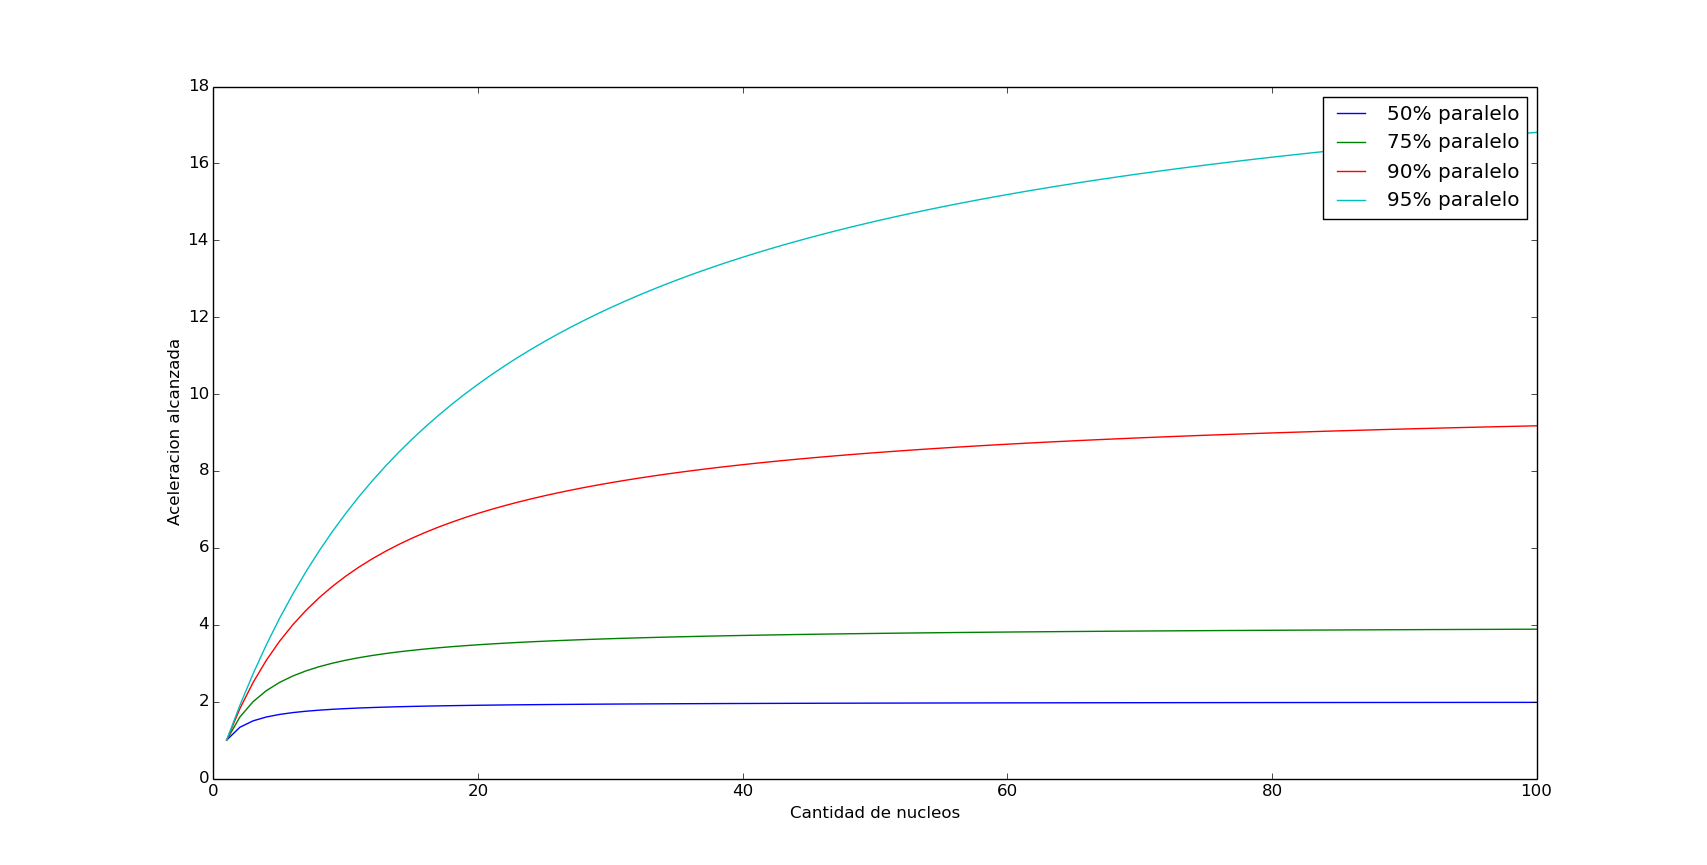
\includegraphics[width=\textwidth]{images/amdahl.png}
    \caption{Aceleraci\'on te\'orica m\'axima (en veces) dada por la ley de Amdahl, seg\'un la cantidad de nucleos de procesamiento}
    \label{fig:amdahl_plot}
\end{figure}

Un ejemplo de esta ley en acci\'on es que si $95 \%$ del problema es paralelizable entonces el l\'imite te\'orico de
mejora es de 20 veces (el programa corriendo sobre infinitos cores se ejecutar\'ia en un veinteavo del tiempo que originalmente
requer\'ia). La curva puede verse graficada en~\ref{fig:amdahl_plot}.

La ley de Amdahl describe el pico teorico de mejora y es una simplificaci\'on, ya que asume que todos los cores tienen
trabajo perfectamente distribuido sin comunicaci\'on entre ellos por motivos de sincronizaci\'on.

Por otro lado, la presencia de un componente com\'un (la memoria) puede introducir cuellos de botella en el acceso a los
datos, ya que si el \textit{bus} de memoria es saturado con pedidos los procesadores deben detener su ejecuci\'on hasta que
los datos est\'en listos, elimin\'andose entonces el procesamiendo paralelo.

Otro elemento de conflicto son los caches. Como los procesadores deben tener una visi\'on unificada y consistente de la
memoria, a veces es necesario que estos coordinen los valores de sus caches, especialmente ante una escritura de memoria.
Esto se conoce como \textit{coherencia de caches} e involucra una sincronizaci\'on serial de alto \textit{overhead}, ya
que implica coordinaci\'on entre dos o m\'as procesadores a trav\'es de un bus de memoria.

Es en este punto que el impacto en el comportamiento del programa puede ser tan fuerte como sutil. Un fen\'omeno que
ilustra esto es el de \textit{false sharing}. Este fen\'omeno ocurre cuando una variable no compartida entre threads
reside en la misma l\'inea de cache con una que si, requiriendo entonces que sea pasada de lado a lado entre cores aunque
nunca fuese esto necesario, da\~nando seriamente la escalabilidad del algoritmo a muchos procesadores y siendo
dificil de descubrir al depender intrinsicamente del sistema en el que se corre.
